\documentclass[ 12pt, xcolor=beamer,table,usenames,dvipsnames, ignorenonframetext, ngerman]{beamer}
\usetheme{Frankfurt}
\usecolortheme{dove}
\usepackage{appendixnumberbeamer}
\setbeamersize{text margin left=20pt,text margin right=20pt,}
\useoutertheme{default}
\beamertemplatenavigationsymbolsempty 
\setbeamertemplate{headline}{}
\setbeamertemplate{itemize item}{\textbullet}

\addtobeamertemplate{navigation symbols}{}{
	\ifnum\insertframenumber>\inserttotalframenumber%
	\relax
	\else%
	\usebeamerfont{footline}%
	\usebeamercolor[fg]{footline}%
	\hspace{1em}%
	\insertframenumber
	\fi%
}
\setbeamercolor{footline}{fg=black}
\setbeamercolor{palette primary}{bg=blue!15,fg=black}
\setbeamercolor{background canvas}{bg=blue!5}
\setbeamercolor{palette secondary}{bg=blue!5}
\setbeamercolor{palette tertiary}{bg=blue!5}
\setbeamercolor{palette quaternary}{bg=blue!5}
\usepackage{soul}
\makeatletter
\let\HL\hl
\renewcommand\hl{%
	\let\set@color\beamerorig@set@color
	\let\reset@color\beamerorig@reset@color
	\HL}

\usepackage{tipa}
\usepackage{tikz}
\usetikzlibrary{shapes.geometric, arrows}
\mode<presentation>

\setbeamercovered{invisible}
\usepackage{multicol}
\usepackage[english]{babel}
\usepackage[latin1]{inputenc}
\usepackage{times}
\usepackage[T1]{fontenc}
\usepackage{ulem}
\usepackage{tipa}
\usepackage{qtree}
\usepackage{phonrule}
\usepackage{graphicx}
\usepackage{apacite}
\usepackage{xcolor}
\setlength\parindent{0pt}
\usepackage{natbib}
\usepackage{tikz}
\usetikzlibrary{arrows.meta}
\usepackage{tcolorbox}
\tcbuselibrary{raster}

\DeclareRobustCommand{\greencheck}{%
	\tikz\fill[scale=0.6, color=ForestGreen]
	(0,.35) -- (.25,0) -- (1,.7) -- (.25,.15) -- cycle;%
}
\title{How do conventions emerge in group communication?}
\author{Veronica Boyce}
\date{CogSci seminar}
\begin{document}

\begin{frame}
\maketitle
\pause
\begin{tikzpicture}[remember picture,overlay]
\node[xshift=1.5cm,yshift=1.2cm] at (current page.south west) {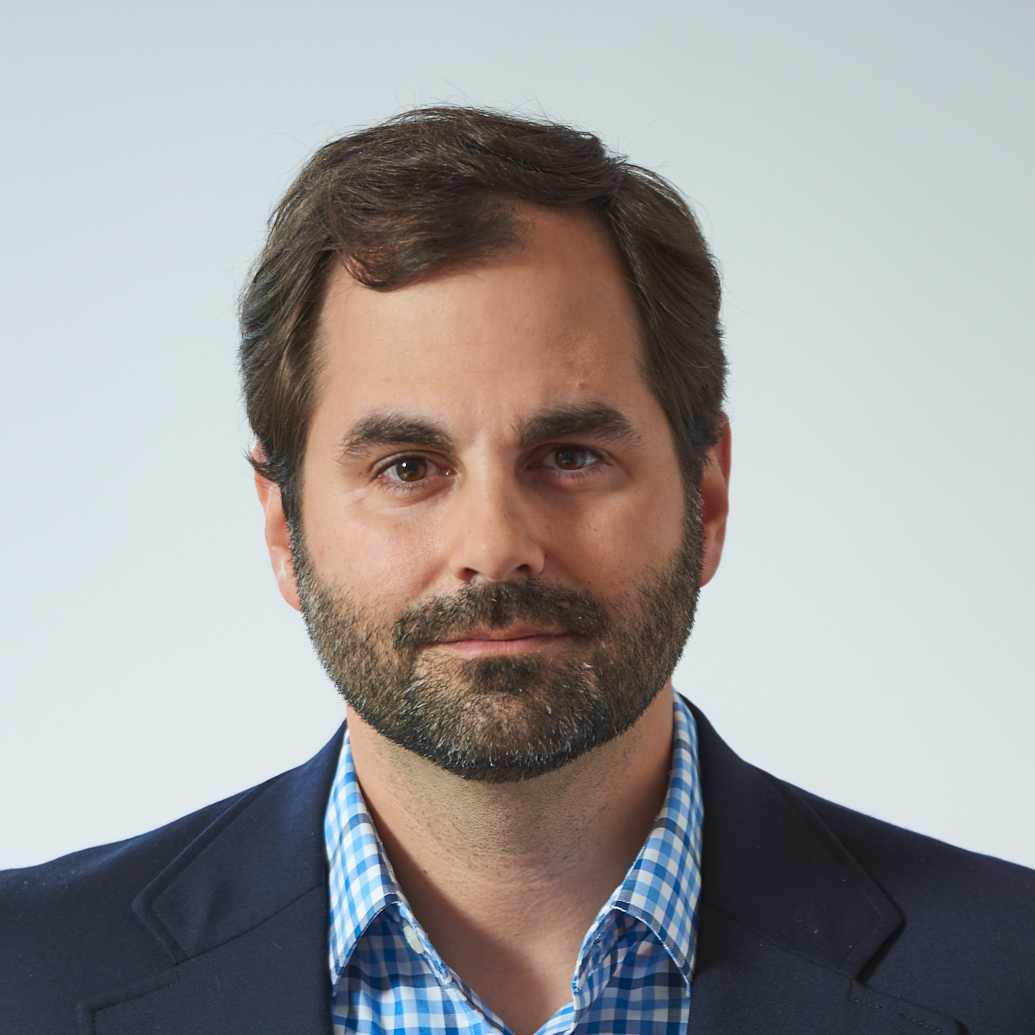
\includegraphics[width=.2\textwidth]{../images/mike.jpg}};
\node[xshift=-2.5cm,yshift=1.2cm] at (current page.south) {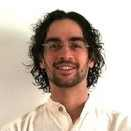
\includegraphics[width=.2\textwidth]{../images/noah.jpg}};
\node[xshift=0cm,yshift=1.2cm] at (current page.south) {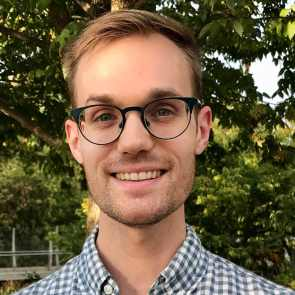
\includegraphics[width=.2\textwidth]{../images/robert.jpeg}};\pause
\node[xshift=-2.5cm,yshift=1.2cm] at (current page.south east) {
\includegraphics[width=.4\textwidth]{../images/hai.jpg}};
\end{tikzpicture}
\end{frame}

\begin{frame}{\large Communication occurs in many contexts}
\pause 

{\large Ranging from one-on-one to small group \\to large group to broadcast}

\pause
\medskip

In all cases, need to efficiently establish reference. 

\end{frame}

\begin{frame}{\large Clark \& Wilkes-Gibbs 1986: Efficient Reference}
	\pause
	\vspace{-.2cm}
	\begin{center}
		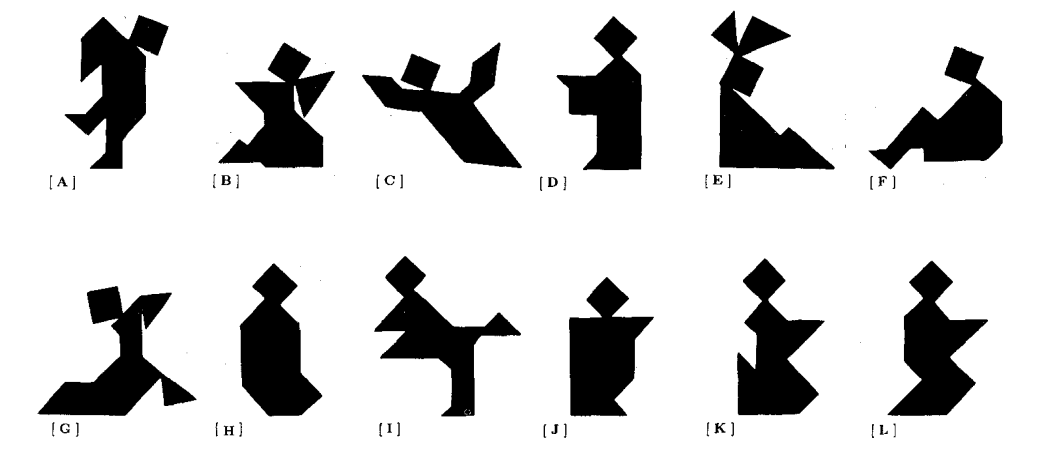
\includegraphics[width=.7\textwidth]{../images/clark_tangrams.png}
	\end{center}
	\vspace{-.4cm}
	\pause
	\begin{small}
		\begin{enumerate}
			\setlength{\itemsep}{-2pt}
			
			\item All right, the next one looks like a person who's ice skating, except, they're sticking two arms out in front. \pause
			\item Um, the next one's the person ice skating that has two arms? \pause
			\item The fourth one is the person ice skating, with two arms. \pause
			\item The next one's the ice skater. \pause
			\item The fourth one's the ice skater. \pause
			\item The ice skater.
		\end{enumerate}
	\end{small}
\end{frame}


\begin{frame}{\large Clark \& Wilkes-Gibbs 1986: Reduction}
	\begin{columns}
		\begin{column}{.55\textwidth}
				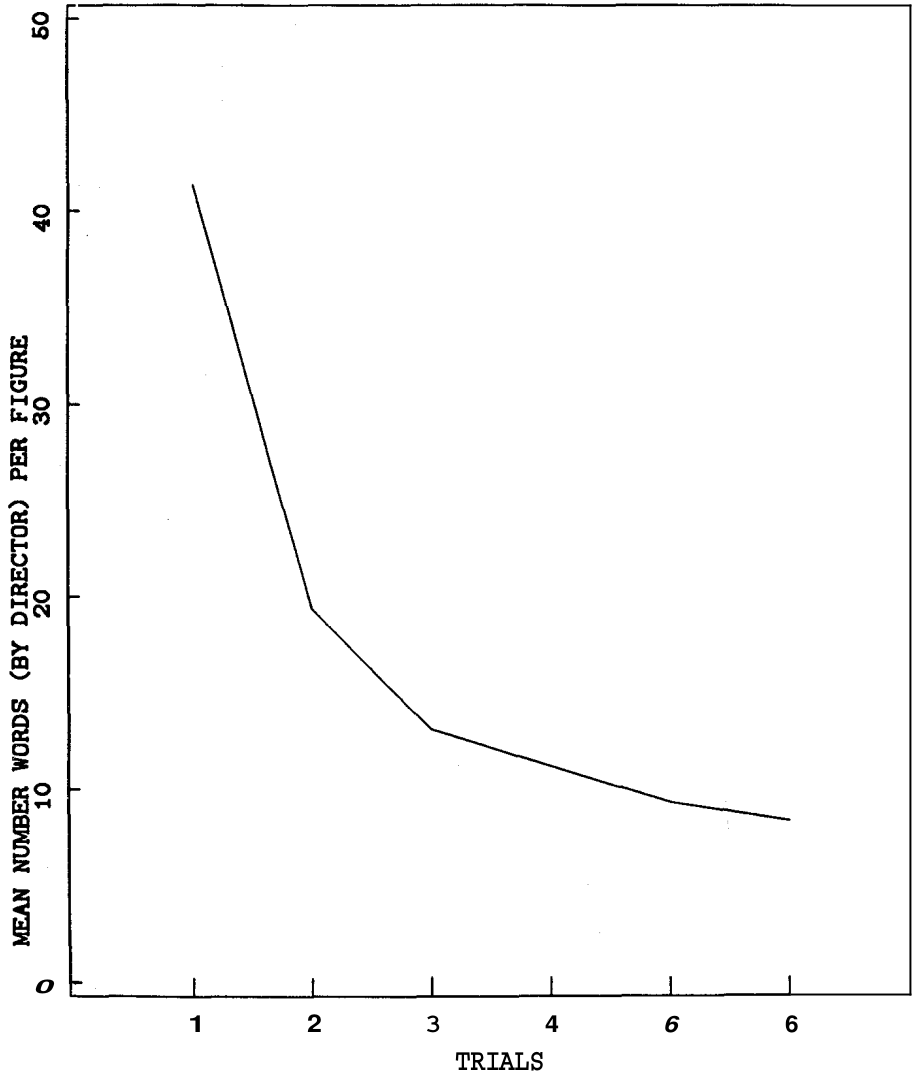
\includegraphics[width=\textwidth]{../images/clark_words.png}
		\end{column}
	\begin{column}{.45\textwidth}
		\pause
		
		Ubiquitous phenomenon
		\smallskip
		
		Many explanations:
		\begin{itemize}
			\item Common ground {\footnotesize (Clark 1996)}
			\item Recursive mentalistic inference  {\footnotesize (Goodman \& Frank 2016)}
			\item Interactive priming {\footnotesize (Garrod \& Pickering 2009)}
		\end{itemize}
	 (Won't address today)
	\end{column}
	\end{columns}
	


	
\end{frame}



%
\begin{frame}{\large Hawkins, Frank, \& Goodman 2020: \\Scaling up via web-based experiments }
\begin{itemize}
	\item Cued version with feedback on each trial 
	\item Message with a chat box 
	\item After all exclusions, 83 dyads 
\end{itemize}
\begin{center}
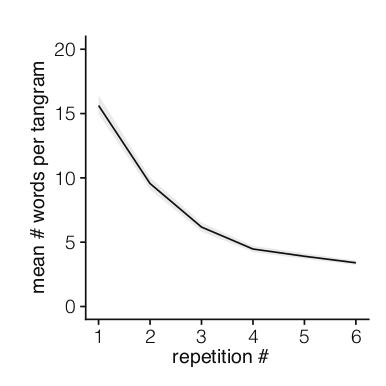
\includegraphics[width=.5\textwidth]{../images/hawkins_fewer_words_square.png}
\end{center}
\end{frame}
%


\begin{frame}{\large Hawkins, Frank, \& Goodman 2020: Content Analysis}
	\begin{center}
	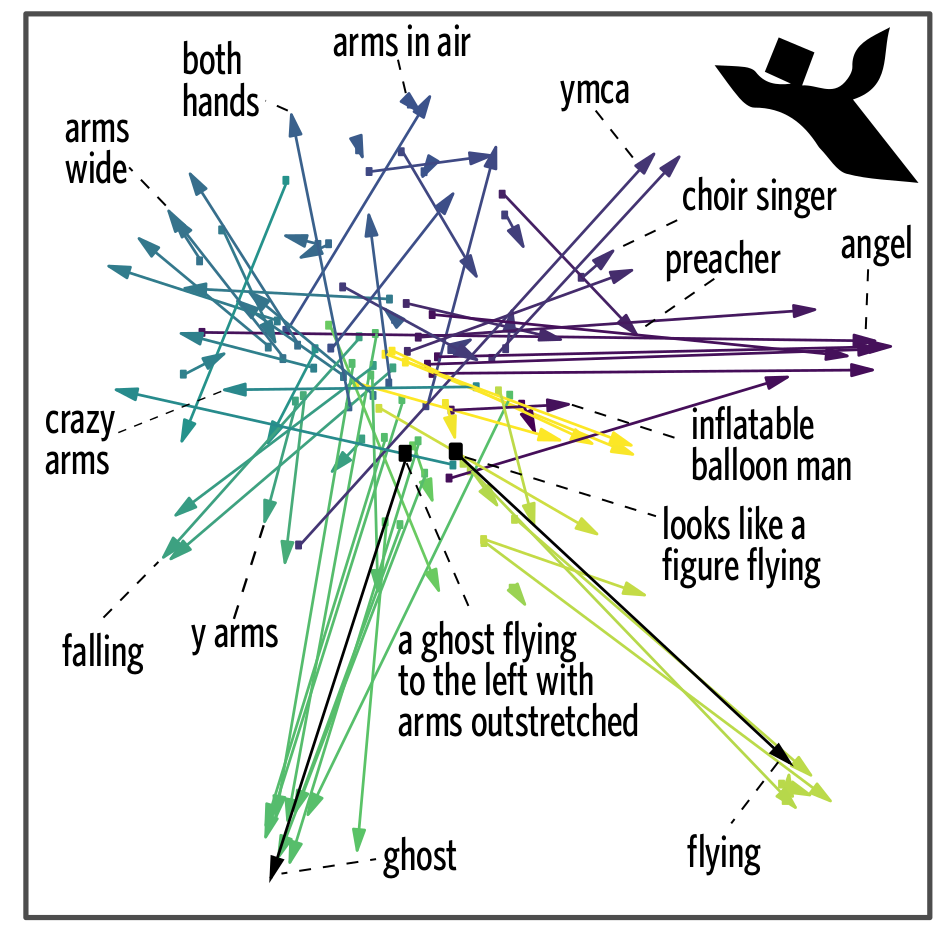
\includegraphics[width=.6\textwidth]{../images/hawkins_semantics.png}
	\end{center}
	Semantics converge within and diverge between groups
\end{frame}

\begin{frame}{}
	\begin{large}
 Dyads are well-studied in this paradigm,...
 \pause
 
  but much real-life communication is not dyadic.

\bigskip

\pause

 How does efficient reference work in groups?
\end{large}
\end{frame}

\begin{frame}{\large Yoon \& Brown-Schmidt 2019: Audience design}
	Speaker trains with some matchers\\
	Then talks with knowledgeable and/or naive listeners
	\medskip
	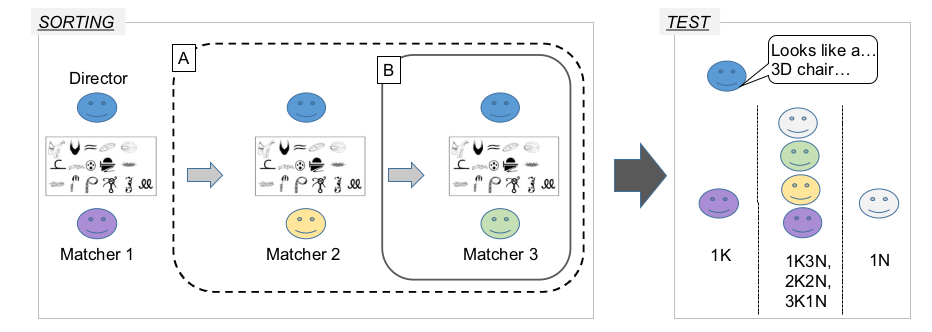
\includegraphics[width=\textwidth]{../images/yoon_diagram.png}
	
	Longer, more elaborated \& disfluent utterances with mixed or naive listeners
	%Mention that these studies were a real tour de force
\end{frame}

\begin{frame}{\large Weber \& Camerer 2003: Adversarially trained listeners}
	
	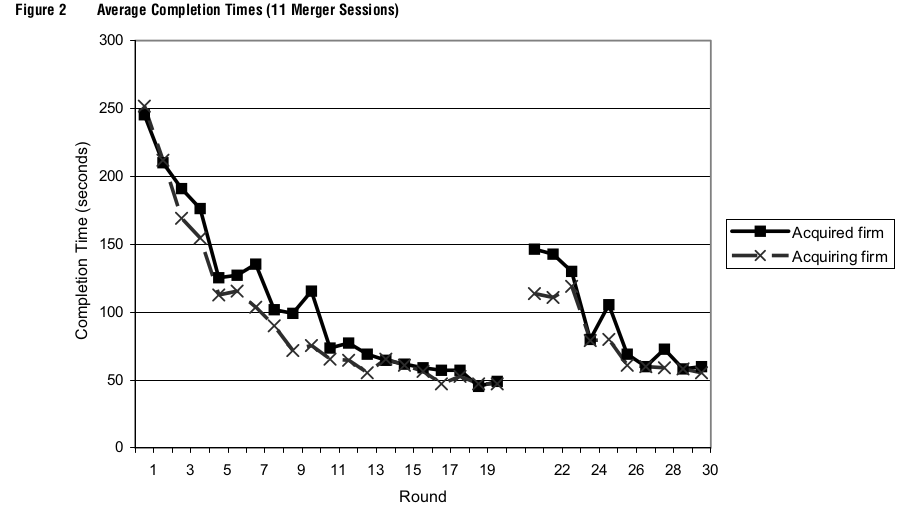
\includegraphics[width=\textwidth]{../images/weber.png}
	Hard to accommodate listeners with different concepts
\end{frame}

\begin{frame}{\large FYP: Communication in small groups}
	Compare groups of 2/3/4 communicators\\
	Follow paradigm of Hawkins et al. (2020)
	\begin{itemize}
		\item Rotate who the speaker is
		\item Different feedback
	\end{itemize} 
Questions we can address:
\begin{itemize}
	\item speed of convergence by group size
	\item managing multiple listeners
	\item use convention v new description
	\item where/when do conventions originate
\end{itemize}

\end{frame}

\begin{frame}{\large Empirica (Almaatouq et al 2020)}
Virtual Lab platform for real-time interactive experiments
%TODO describe what this is
 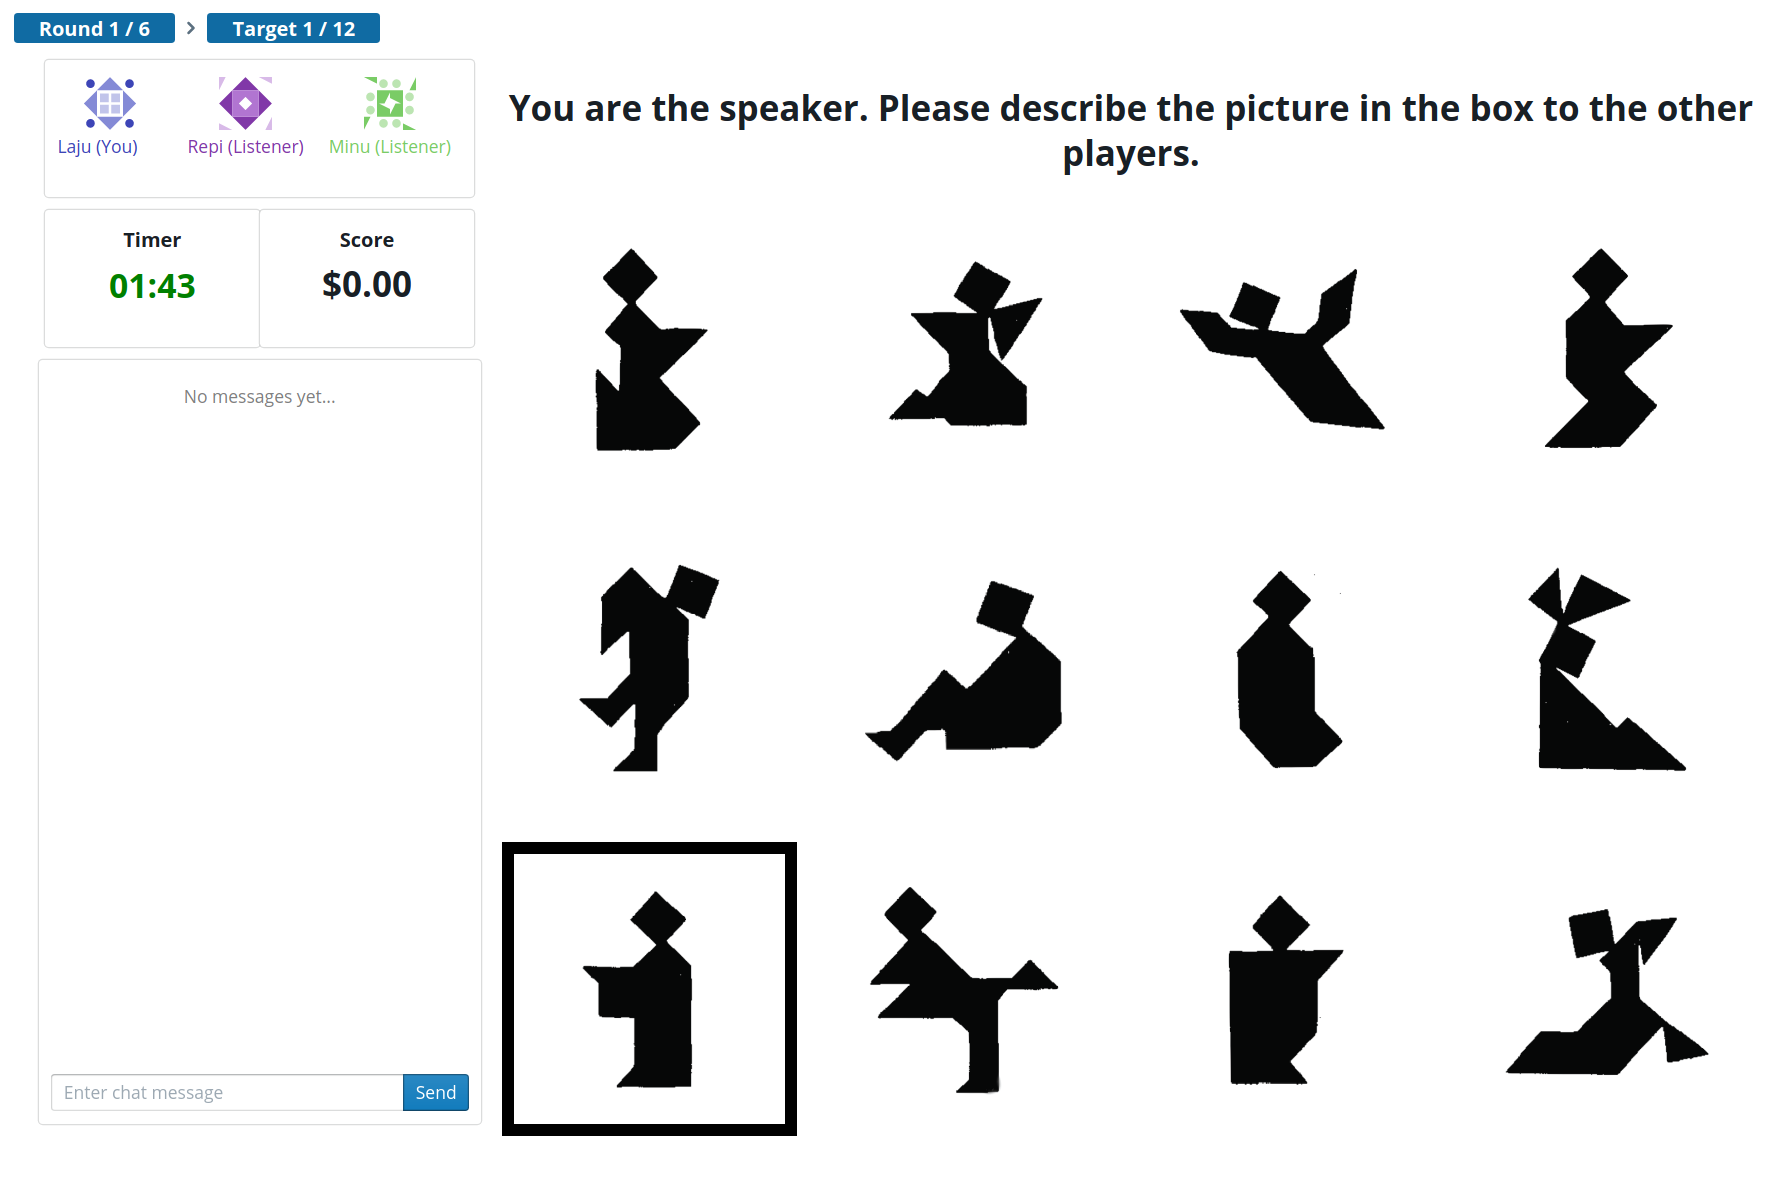
\includegraphics[width=\textwidth]{../images/interface.PNG}
\end{frame}

\begin{frame}{Experiment Framework}
	\only<1>{\begin{tikzpicture}[remember picture,overlay]
	\node[] at (current page.center) {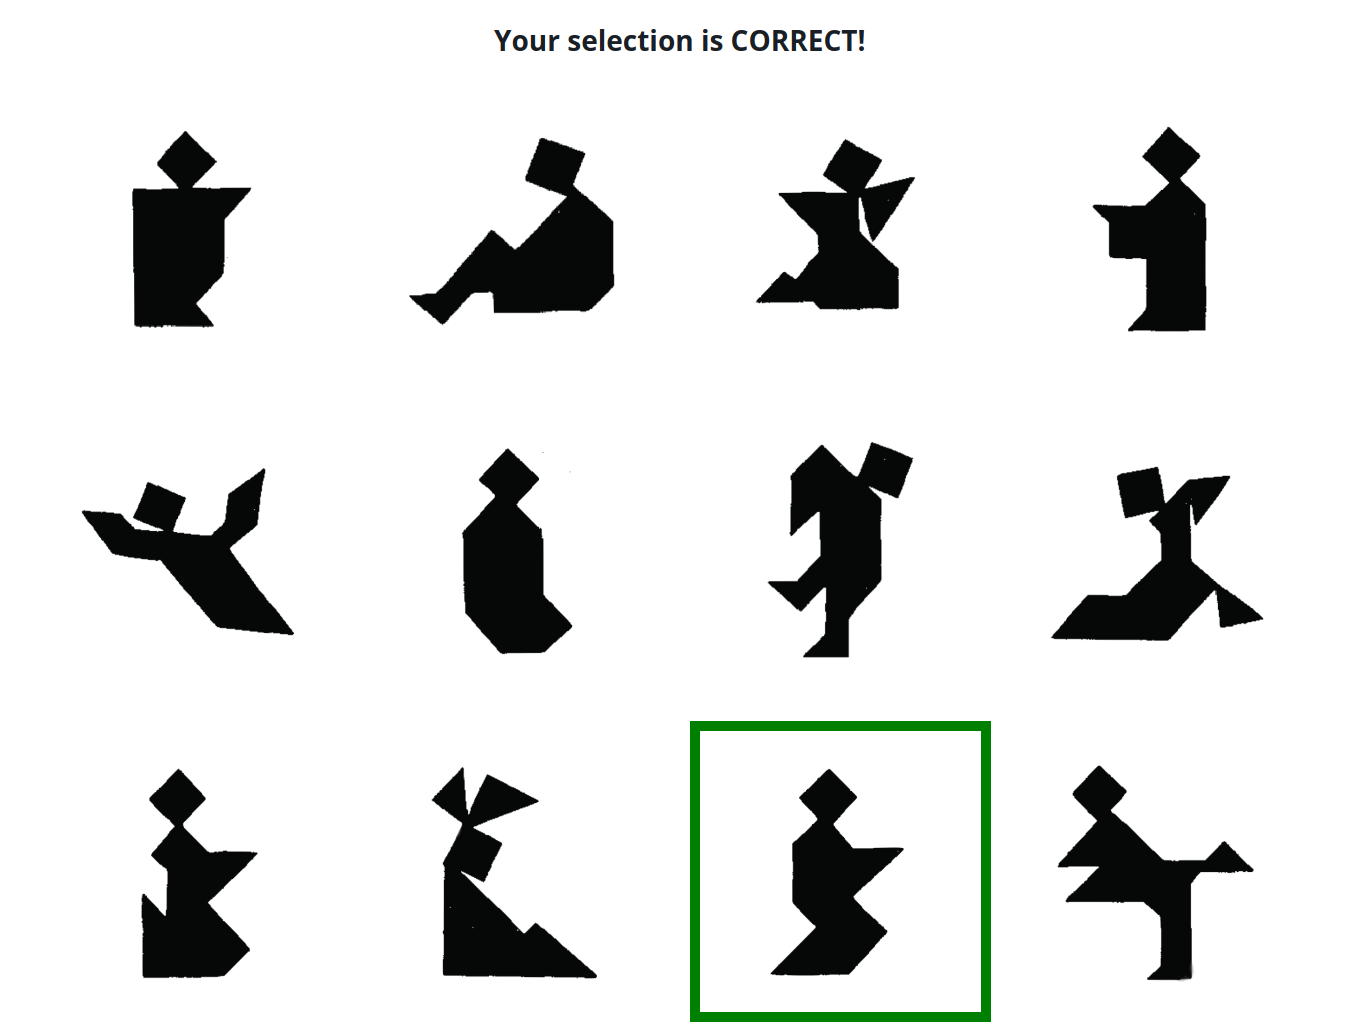
\includegraphics[width=.8\textwidth]{../images/listener_correct.png}};
		\node[yshift=1cm] at (current page.south) {Bonus: 4 points};
		\end{tikzpicture}}
\only<2>{\begin{tikzpicture}[remember picture,overlay]
\node[] at (current page.center) {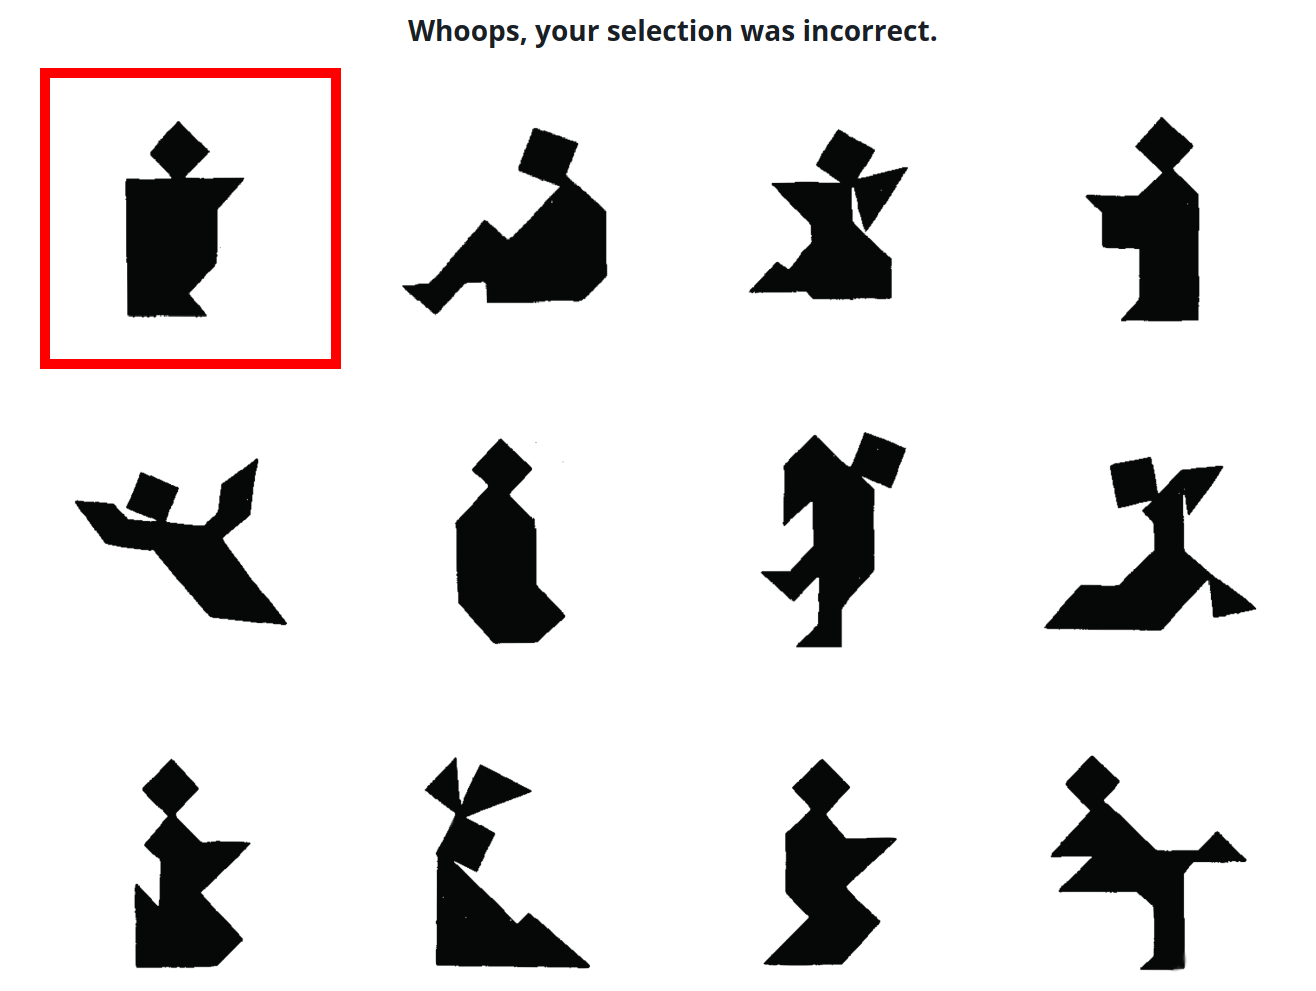
\includegraphics[width=.8\textwidth]{../images/listener_wrong.png}};
			\node[yshift=1cm] at (current page.south) {Bonus: 0 points};
			\end{tikzpicture}}
\only<3>{\begin{tikzpicture}[remember picture,overlay]
	\node[] at (current page.center) {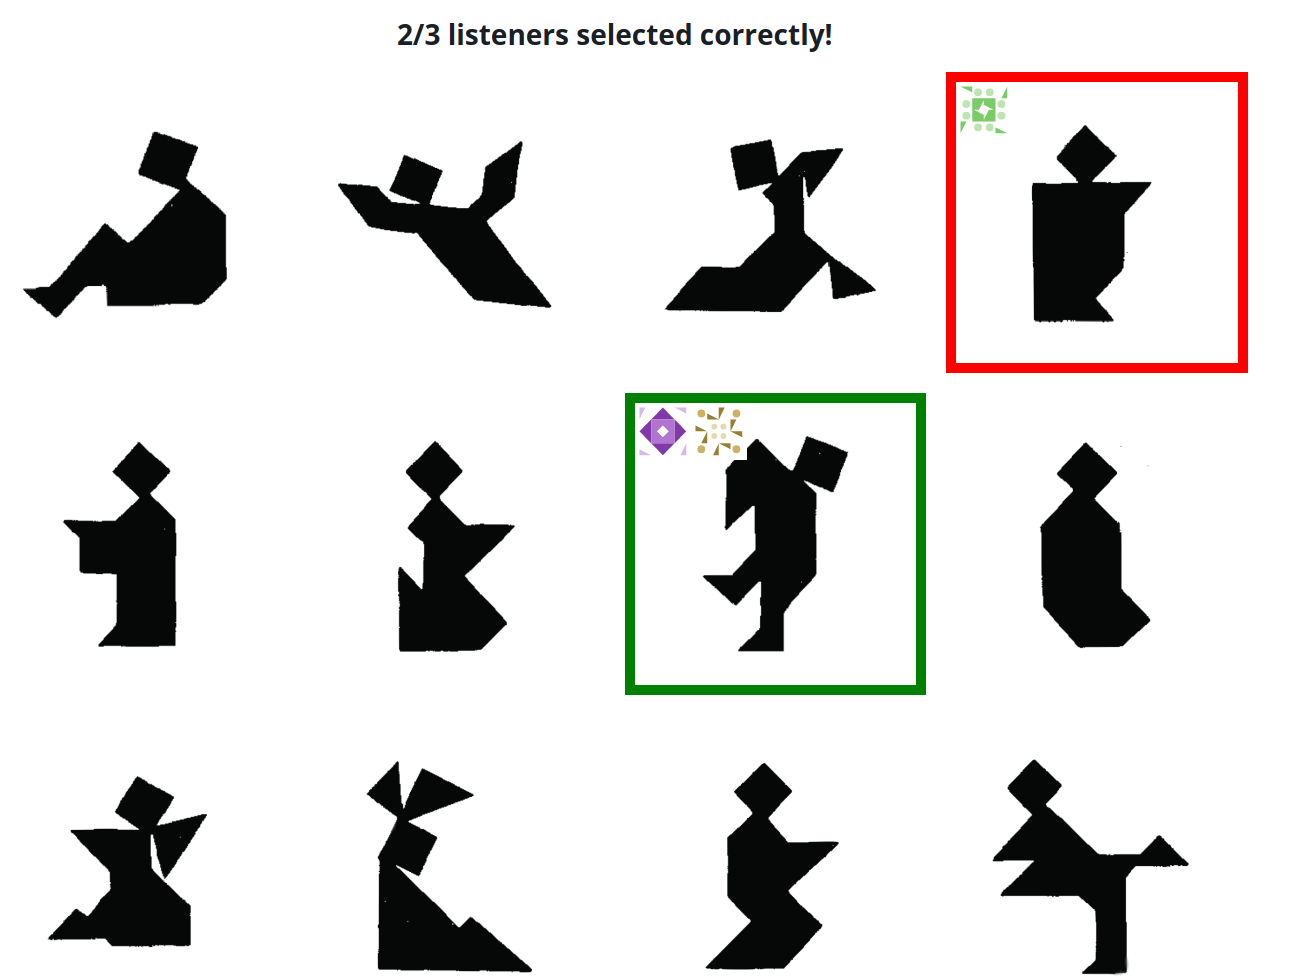
\includegraphics[width=.8\textwidth]{../images/speaker_feedback.png}};
\node[yshift=1cm] at (current page.south) {Bonus: Average of listeners = (2/3) * 4 points};

	\end{tikzpicture}}
\end{frame}
\begin{frame}{\large Recruitment}
	Goal: 20 games in each of 2/3/4-player conditions
	
	Each game has 6 blocks of 12 tangrams\pause
	
	\medskip
	
	Actual recruitment (over 3 days):
	\begin{itemize}
		\item 15 2-player games (+ 4 partial)
		\item 18 3-player games (+ 2 partial)
		\item 20 4-player games (+ 1 partial)
	\end{itemize}
Include all complete blocks

\end{frame}


\begin{frame}{\large Results:  Accuracy is high and increasing}
	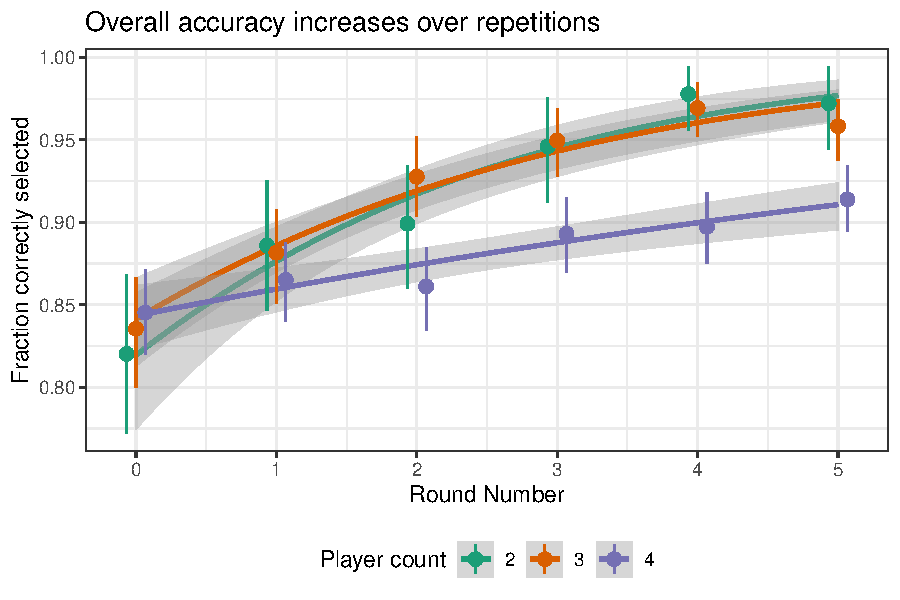
\includegraphics[width=\textwidth]{../images/accuracy.pdf}

\end{frame}

\begin{frame}{\large Results: 	Faster in later rounds}
	
	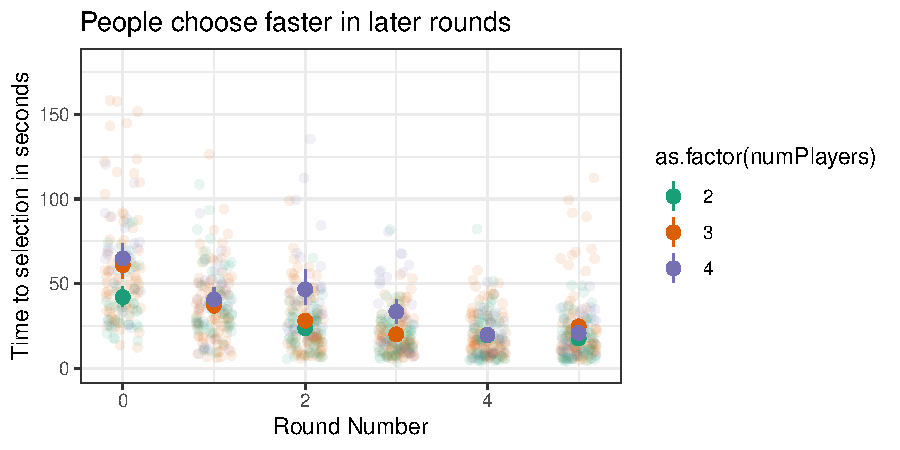
\includegraphics[width=\textwidth]{../images/time.pdf}


\end{frame}

\begin{frame}{\large Results: Reduction in words over time}
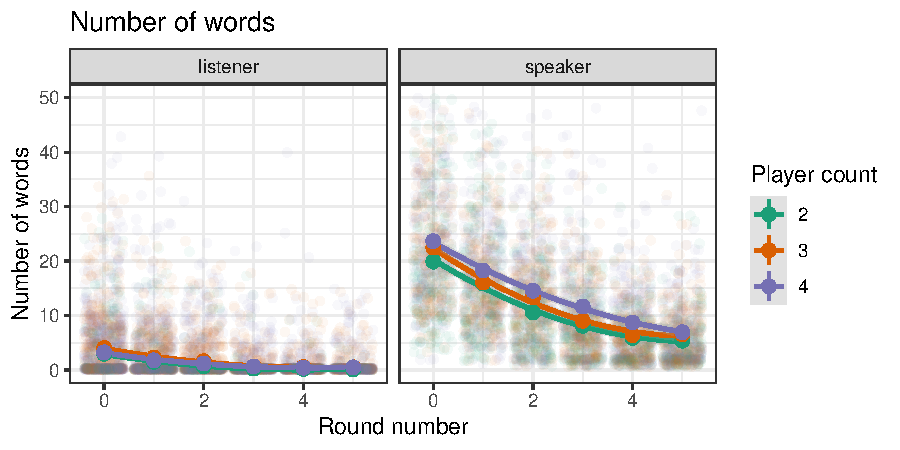
\includegraphics[width=\textwidth]{../images/words.pdf}


\end{frame}

\begin{frame}{\large Results: Variability in reduction rate}
	Most groups/tangrams reduce gradually
	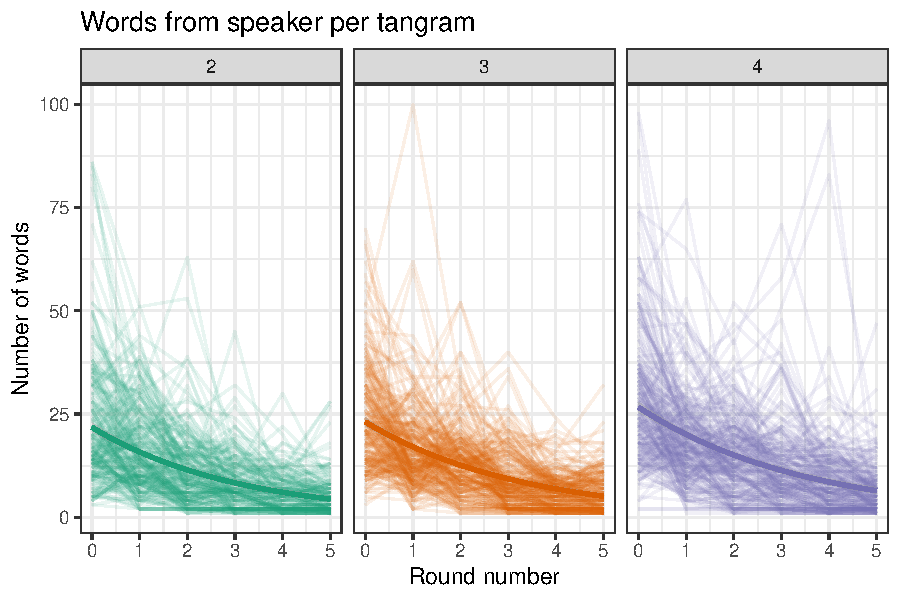
\includegraphics[width=\textwidth]{../images/words_lines.pdf}
\end{frame}

\begin{frame}{\large Results: Tangrams vary in nameability}
	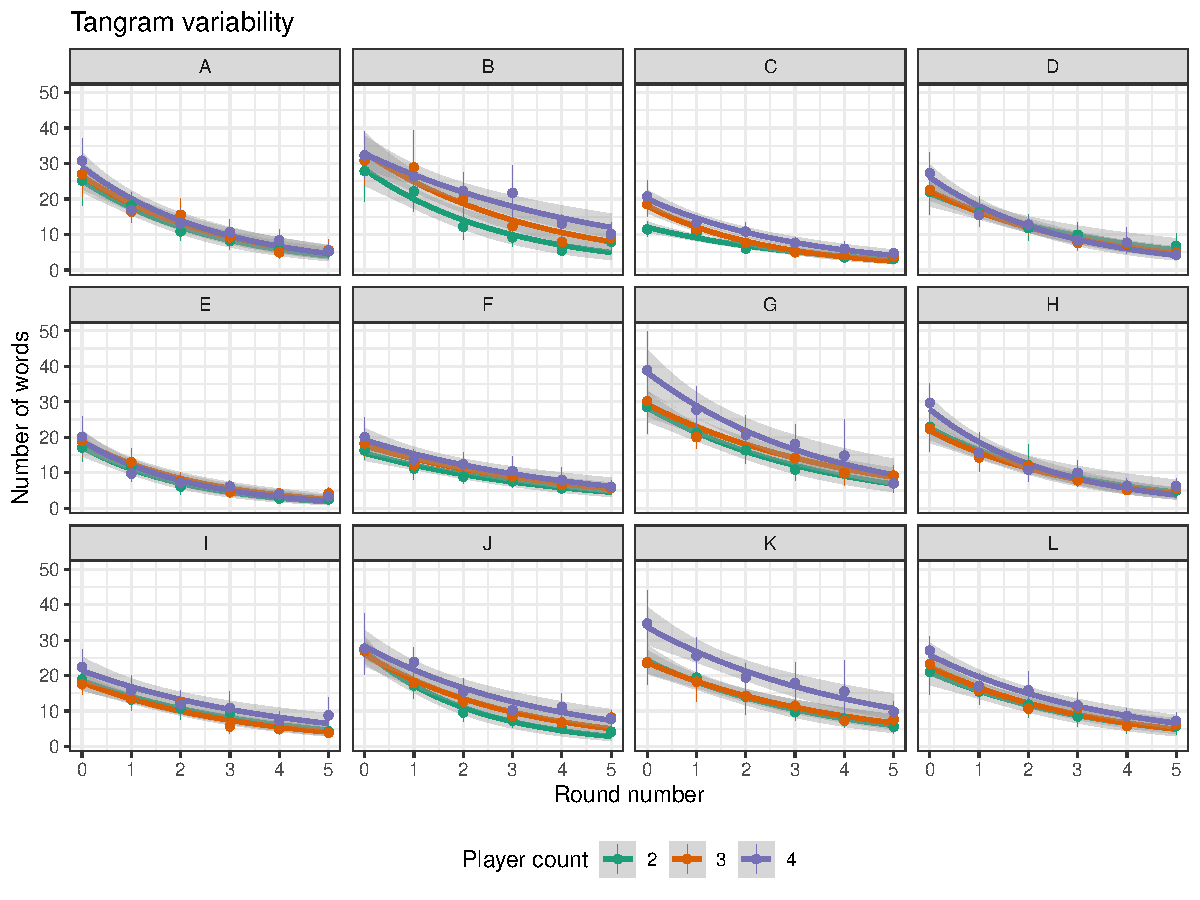
\includegraphics[width=\textwidth]{../images/words_tangrams.pdf}
\end{frame}

\begin{frame}{\large Results: Models}
	Bayesian model to allow for correlated variability
	\begin{itemize}
		\item Block: -3.22 words [-4.95, -1.55]
		\item Player count: 1.93 words [ -0.15, 4.02]
		\item Speaker choosing wrong on the previous block: 4.15 words [2.54, 5.79]
	\end{itemize}

	\end{frame}

\begin{frame}{\large Example: iBaby}
	\begin{tikzpicture}[remember picture,overlay]
	\node[xshift=-1.5cm,yshift=-3cm] at (current page.north east) 
	{
\includegraphics[width=.2\textwidth]{../images/tangram_H.png}};
	\end{tikzpicture}
	
		\begin{enumerate}
			\setlength{\itemsep}{-2pt}
			\item A(S):Looks like a letter 'i'\\
			C: does it look like with its hand out or not\\
			B: \^{}\\
			A(S): no hand it is just a head and a body.\\
			C: oke\\
			A(S): more like a baby that has been swaddled in a blanket\\
			\item B(S): swaddled baby\\
			B(S): I\\
			B(S): i\\
			\item C(S): the baby i \\
			\item D(S): baby swaddled, looks like an i\\
			\item A(S): swaddled baby\\
			\item B(S): iBaby
		\end{enumerate}

\end{frame}


\begin{frame}{\large Example: Skydiving ghost superman}
	\begin{tikzpicture}[remember picture,overlay]
	\node[xshift=-1.5cm,yshift=-3cm] at (current page.north east) 
	{
\includegraphics[width=.2\textwidth]{../images/tangram_C.png}};
	\end{tikzpicture}
	\begin{enumerate}
		\setlength{\itemsep}{-2pt}
		\item A(S):flying man\\
		A(S): like superman \\
		A(S): hands in the air\\
		A(S): like skydiving
		\item B(S): the diver with no legs\\
		A: ok
		\item C(S): This one looks like a ghost to me, but you called it superman or skydiver\\
		A: ok no legs?\\
		C(S): Correct\\
		A: ok
		\item A(S): ghost, superman, skydiver
		\item B(S): sky diver, ghost\\
		A: ok\\
		\item C(S): Skydiving ghost superman
	\end{enumerate}
	
\end{frame}

\begin{frame}{\large Example: Karate kid}
	\begin{tikzpicture}[remember picture,overlay]
	\node[xshift=-1.5cm,yshift=-3cm] at (current page.north east) 
	{
\includegraphics[width=.2\textwidth]{../images/tangram_A.png}};
	\end{tikzpicture}
	\begin{enumerate}
		\setlength{\itemsep}{-2pt}
		\item A(S): Similar to the karate kid movie\\
		A(S): the crane kick\\
		B: Haha! Does it look like they have dangly sleeves!\\
		C: I don't know that one.\\
		A(S): yes\\
		D:yes i see, thats a good explenation.\\
	\end{enumerate}
	
\end{frame}

\begin{frame}{\large Example: Lack of shorthand}
	\begin{tikzpicture}[remember picture,overlay]
	\node[xshift=-.5cm,yshift=-2cm] at (current page.north east) 
	{
\includegraphics[width=.2\textwidth]{../images/tangram_J.png}};
	\end{tikzpicture}
	\vspace{-20pt}
	\begin{footnotesize}
	\begin{enumerate}
		\setlength{\itemsep}{-2pt}
		\item A(S):Diamond on top. Body with no real arms or legs. The body is shaped like a boot with the diamond on top.\\
		C: Is the boot pointed left or right?\\
		
		\item B(S): diamond on top, large body beneath it. Left is a straight line all the way down, small variations on the right to the main body\\
		\item C(S): Diamond in center on top. Left side straight, right side carved out like a vase.\\
		\item D(S): Diamond head, flat topped body, straight on the left side with two triangles pointing out on the left\\
		D(S): *on the right\\
		\item A(S): Diamond on top. Left side is straight, right side is obstructed, looks like a boot\\
		B: what do you mean by obstructed?\\
		A(S): The left side of the body is right, right side has bents in it	\\
		\item B(S): Diamond on top of a long large body/rectangle. Left side is complete, right side has bits missing
	\end{enumerate}
	\end{footnotesize}
\end{frame}



\begin{frame}{\large Example: Meta doesn't always help}
	\begin{tikzpicture}[remember picture,overlay]
	\node[xshift=-1cm,yshift=-2cm] at (current page.north east) 
	{
\includegraphics[width=.2\textwidth]{../images/tangram_L.png}};
	\end{tikzpicture}
	\vspace{-20pt}
	\begin{footnotesize}
		\begin{enumerate}
			\setlength{\itemsep}{-2pt}
			\item ...A(S): yes, the legs are like a zig zag\\
			C: CODE name ZIGZAG	\\
			A(S):	There are no legs upwards
			\item B(S): okay so similar to begger guy but no foot pointing up\\
			B(S): its like a zigzag\\
			B(S): i forgot the code name\\
			D: zigzag yea\\
			A: The one standing with knees bent\\
			B(S): yeah\\
			B(S): standing \\
			C: Yeah zigzag
			\item C(S):	The begger with no foot coming out from the left\\
			B: zigzag\\
			C(S):	zigzag it is\\
			C(S):	sorry i forgot\\
			\item D(S):	zigzag
			\item A(S):	zigzag	
			\item B(S):	beggar guy\\
			B(S): zigzag
			
		\end{enumerate}
	\end{footnotesize}
\end{frame}
\begin{frame}{\large Future analyses: Semantics}
		\begin{tikzpicture}[remember picture,overlay]
	\node[xshift=-2.5cm,yshift=-3.2cm] at (current page.north east) 
		{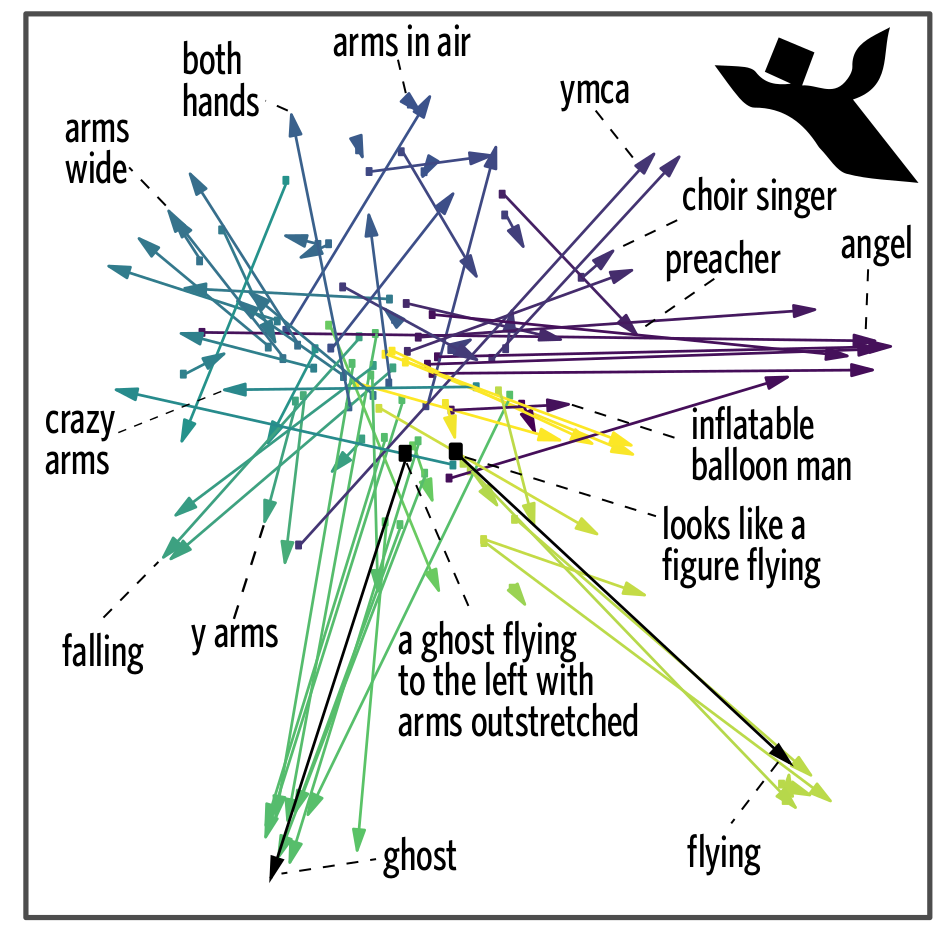
\includegraphics[width=.4\textwidth]{../images/hawkins_semantics.png}};
	\end{tikzpicture}

	\begin{itemize}
		\item Convergence by group size
		\item Accuracy \& convergence
		\item Geometric v metaphorical language
		\item Where/when are (atypical) concepts introduced?
	\end{itemize}
\pause
	\begin{tikzpicture}[remember picture,overlay]
\node[yshift=2cm] at (current page.south) 
{
\includegraphics[width=.2\textwidth]{../images/tangram_C.png}};
\end{tikzpicture}
\end{frame}


\begin{frame}{\large Future directions} 
\pause
How far does this generalize?
 \begin{itemize}
 	\item Group size
 	\item Stimuli
 	\item Game set ups, feedback
 \end{itemize}
	\pause
What makes communication more efficient?
\begin{itemize}
	\item Shared expertise
	\item Curriculum learning
\end{itemize}
\pause 
Online implementation makes iterations, variations easy
\end{frame}

\begin{frame}{\large Comments, Questions?}
	Looking for feedback on
	\smallskip
	\begin{itemize}
	\item Analyses
	\item Future data sets
	\end{itemize}
\end{frame}

\appendix

%\begin{frame}{Hawkins, Frank, \& Goodman 2020}
%	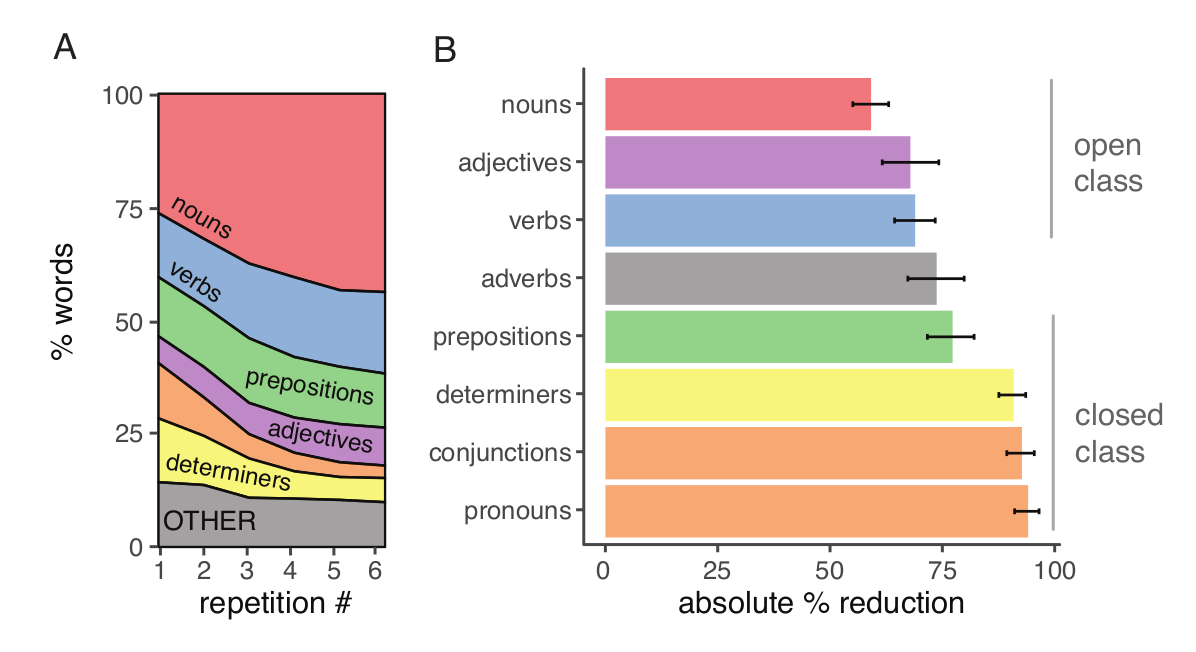
\includegraphics[width=\textwidth]{../images/hawkins_pos.png}
%	Words tend to drop out in syntactic units
%\end{frame}
\end{document}

